%%%%%%%%%%%%%%%%%%%%%%%%%%%%%%%%%%%%%%%%%
% Masters/Doctoral Thesis 
% LaTeX Template
% Version 2.5 (27/8/17)
%
% This template was downloaded from:
% http://www.LaTeXTemplates.com
%
% Version 2.x major modifications by:
% Vel (vel@latextemplates.com)
%
% This template is based on a template by:
% Steve Gunn (http://users.ecs.soton.ac.uk/srg/softwaretools/document/templates/)
% Sunil Patel (http://www.sunilpatel.co.uk/thesis-template/)
%
% Template license:
% CC BY-NC-SA 3.0 (http://creativecommons.org/licenses/by-nc-sa/3.0/)
%
%%%%%%%%%%%%%%%%%%%%%%%%%%%%%%%%%%%%%%%%%

%----------------------------------------------------------------------------------------
%	PACKAGES AND OTHER DOCUMENT CONFIGURATIONS
%----------------------------------------------------------------------------------------

\documentclass[
11pt, % The default document font size, options: 10pt, 11pt, 12pt
%oneside, % Two side (alternating margins) for binding by default, uncomment to switch to one side
english, % ngerman for German
singlespacing, % Single line spacing, alternatives: onehalfspacing or doublespacing
%draft, % Uncomment to enable draft mode (no pictures, no links, overfull hboxes indicated)
%nolistspacing, % If the document is onehalfspacing or doublespacing, uncomment this to set spacing in lists to single
%liststotoc, % Uncomment to add the list of figures/tables/etc to the table of contents
%toctotoc, % Uncomment to add the main table of contents to the table of contents
%parskip, % Uncomment to add space between paragraphs
%nohyperref, % Uncomment to not load the hyperref package
headsepline, % Uncomment to get a line under the header
%chapterinoneline, % Uncomment to place the chapter title next to the number on one line
%consistentlayout, % Uncomment to change the layout of the declaration, abstract and acknowledgements pages to match the default layout
]{MastersDoctoralThesis} % The class file specifying the document structure

\usepackage[utf8]{inputenc} % Required for inputting international characters
\usepackage[T1]{fontenc} % Output font encoding for international characters

\usepackage{mathpazo} % Use the Palatino font by default

%\usepackage[backend=bibtex,style=authoryear,natbib=true]{biblatex} % Use the bibtex backend with the authoryear citation style (which resembles APA)

\usepackage[backend=bibtex]{biblatex}

\addbibresource{example.bib} % The filename of the bibliography

\usepackage[autostyle=true]{csquotes} % Required to generate language-dependent quotes in the bibliography

\usepackage{graphicx} % Image Package
\usepackage{wrapfig}
\graphicspath{ {./Figures/} }

\usepackage{algorithm} % 2 packages to write pseudocode
\usepackage[noend]{algpseudocode}
% Algorithmic modifications
\makeatletter
\newcommand{\ALOOP}[1]{\ALC@it\algorithmicloop\ #1%
	\begin{ALC@loop}}
	\newcommand{\ENDALOOP}{\end{ALC@loop}\ALC@it\algorithmicendloop}
\renewcommand{\algorithmicrequire}{\textbf{Input:}}
\renewcommand{\algorithmicensure}{\textbf{Output:}}
\newcommand{\algorithmicbreak}{\textbf{break}}
\newcommand{\BREAK}{\STATE \algorithmicbreak}
\makeatother

%----------------------------------------------------------------------------------------
%	MARGIN SETTINGS
%----------------------------------------------------------------------------------------

\geometry{
	paper=a4paper, % Change to letterpaper for US letter
	inner=2.5cm, % Inner margin
	outer=3.8cm, % Outer margin
	bindingoffset=.5cm, % Binding offset
	top=1.5cm, % Top margin
	bottom=1.5cm, % Bottom margin
	%showframe, % Uncomment to show how the type block is set on the page
}

%----------------------------------------------------------------------------------------
%	THESIS INFORMATION
%----------------------------------------------------------------------------------------

\thesistitle{Automatic Sychronisation of Subtitle Track With Live Audio} % Your thesis title, this is used in the title and abstract, print it elsewhere with \ttitle
\supervisor{Dr. R\'emi \textsc{Emonet}} % Your supervisor's name, this is used in the title page, print it elsewhere with \supname
%\examiner{} % Your examiner's name, this is not currently used anywhere in the template, print it elsewhere with \examname
\degree{Masters in Machine Learning \& Data Mining} % Your degree name, this is used in the title page and abstract, print it elsewhere with \degreename
\author{Joshua \textsc{Fenech}} % Your name, this is used in the title page and abstract, print it elsewhere with \authorname
%\addresses{} % Your address, this is not currently used anywhere in the template, print it elsewhere with \addressname

%\subject{Biological Sciences} % Your subject area, this is not currently used anywhere in the template, print it elsewhere with \subjectname
%\keywords{} % Keywords for your thesis, this is not currently used anywhere in the template, print it elsewhere with \keywordnames
\university{\href{https://www.univ-st-etienne.fr/fr/index.html}{Universit\'e de Jean Monnet}} % Your university's name and URL, this is used in the title page and abstract, print it elsewhere with \univname
\department{\href{https://mldm.univ-st-etienne.fr/}{MLDM}} % Your department's name and URL, this is used in the title page and abstract, print it elsewhere with \deptname
%\group{\href{http://researchgroup.university.com}{Research Group Name}} % Your research group's name and URL, this is used in the title page, print it elsewhere with \groupname
%\faculty{\href{http://faculty.university.com}{Faculty Name}} % Your faculty's name and URL, this is used in the title page and abstract, print it elsewhere with \facname

\AtBeginDocument{
\hypersetup{pdftitle=\ttitle} % Set the PDF's title to your title
\hypersetup{pdfauthor=\authorname} % Set the PDF's author to your name
\hypersetup{pdfkeywords=\keywordnames} % Set the PDF's keywords to your keywords
}

\begin{document}

\frontmatter % Use roman page numbering style (i, ii, iii, iv...) for the pre-content pages

\pagestyle{plain} % Default to the plain heading style until the thesis style is called for the body content

%----------------------------------------------------------------------------------------
%	TITLE PAGE
%----------------------------------------------------------------------------------------

\begin{titlepage}
\begin{center}

\vspace*{.06\textheight}
{\scshape\LARGE \univname\par}\vspace{1.5cm} % University name
\textsc{\Large Masters 1 Thesis}\\[0.5cm] % Thesis type

\HRule \\[0.4cm] % Horizontal line
{\huge \bfseries \ttitle\par}\vspace{0.4cm} % Thesis title
\HRule \\[1.5cm] % Horizontal line
 
\begin{minipage}[t]{0.4\textwidth}
\begin{flushleft} \large
\emph{Author:}\\
\href{https://www.linkedin.com/in/joshua-fenech-53612471/}{\authorname} % Author name - remove the \href bracket to remove the link
\end{flushleft}
\end{minipage}
\begin{minipage}[t]{0.4\textwidth}
\begin{flushright} \large
\emph{Supervisor:} \\
\href{https://home.heeere.com/}{\supname} % Supervisor name - remove the \href bracket to remove the link  
\end{flushright}
\end{minipage}\\[3cm]
 
\vfill

\large \textit{A thesis submitted in fulfillment of the requirements\\ for the degree of \degreename}\\[0.3cm] % University requirement text
%\textit{in the}\\[0.4cm]
%\groupname\\\deptname\\[2cm] % Research group name and department name
 
\vfill

{\large \today}\\[4cm] % Date
%\includegraphics{Logo} % University/department logo - uncomment to place it
 
\vfill
\end{center}
\end{titlepage}

%----------------------------------------------------------------------------------------
%	DECLARATION PAGE
%----------------------------------------------------------------------------------------

\begin{declaration}
\addchaptertocentry{\authorshipname} % Add the declaration to the table of contents
\noindent I, \authorname, declare that this thesis titled, \enquote{\ttitle} and the work presented in it are my own. I confirm that:

\begin{itemize} 
\item This work was done wholly or mainly while in candidature for a research degree at this University.
\item Where any part of this thesis has previously been submitted for a degree or any other qualification at this University or any other institution, this has been clearly stated.
\item Where I have consulted the published work of others, this is always clearly attributed.
\item Where I have quoted from the work of others, the source is always given. With the exception of such quotations, this thesis is entirely my own work.
\item I have acknowledged all main sources of help.
\item Where the thesis is based on work done by myself jointly with others, I have made clear exactly what was done by others and what I have contributed myself.\\
\end{itemize}
 
\noindent Signed: Joshua Fenech\\
\rule[0.5em]{25em}{0.5pt} % This prints a line for the signature
 
\noindent Date:\\
\rule[0.5em]{25em}{0.5pt} % This prints a line to write the date
\end{declaration}

\cleardoublepage

%----------------------------------------------------------------------------------------
%	ABSTRACT PAGE
%----------------------------------------------------------------------------------------

\begin{abstract}
\addchaptertocentry{\abstractname} % Add the abstract to the table of contents
Subtitle availability is distinctly lacking in cinemas, limiting access to people who are hard of hearing and from minority groups. Whilst technologies are readily available they are rarely implemented, hence there is motivation to devise a technique to enable users to independently access subtitles on their personal devices and synchronise them with minimum difficulty. In order to do so, subtitles were used to create an objective array identifying whether subtitles are present, and this was used to train a convolutional neural network based on the work of \cite{Sabater_2017}. Initial results of 83\% after tuning were boosted to 93\% by swapping the activation and batch normalisation layers. However, further analysis of results indicates varied results. An array matching method was also proposed in order to provide alignment in real time, but this requires further testing and development.
\end{abstract}

%----------------------------------------------------------------------------------------
%	ACKNOWLEDGEMENTS
%----------------------------------------------------------------------------------------

%\begin{acknowledgements}
%\addchaptertocentry{\acknowledgementname} % Add the acknowledgements to the table of contents
%The acknowledgments and the people to thank go here, don't forget to include your project advisor\ldots
%\end{acknowledgements}

%----------------------------------------------------------------------------------------
%	LIST OF CONTENTS/FIGURES/TABLES PAGES
%----------------------------------------------------------------------------------------

\tableofcontents % Prints the main table of contents

\listoffigures % Prints the list of figures

%\listoftables % Prints the list of tables

%----------------------------------------------------------------------------------------
%	ABBREVIATIONS
%----------------------------------------------------------------------------------------

%\begin{abbreviations}{ll} % Include a list of abbreviations (a table of two columns)

%\textbf{LAH} & \textbf{L}ist \textbf{A}bbreviations \textbf{H}ere\\
%\textbf{WSF} & \textbf{W}hat (it) \textbf{S}tands \textbf{F}or\\

%\end{abbreviations}

%----------------------------------------------------------------------------------------
%	PHYSICAL CONSTANTS/OTHER DEFINITIONS
%----------------------------------------------------------------------------------------

%\begin{constants}{lr@{${}={}$}l} % The list of physical constants is a three column table

% The \SI{}{} command is provided by the siunitx package, see its documentation for instructions on how to use it

%Speed of Light & $c_{0}$ & \SI{2.99792458e8}{\meter\per\second} (exact)\\
%Constant Name & $Symbol$ & $Constant Value$ with units\\

%\end{constants}

%----------------------------------------------------------------------------------------
%	SYMBOLS
%----------------------------------------------------------------------------------------

%\begin{symbols}{lll} % Include a list of Symbols (a three column table)

%$a$ & distance & \si{\meter} \\
%$P$ & power & \si{\watt} (\si{\joule\per\second}) \\
%Symbol & Name & Unit \\

%\addlinespace % Gap to separate the Roman symbols from the Greek

%$\omega$ & angular frequency & \si{\radian} \\

%\end{symbols}

%----------------------------------------------------------------------------------------
%	DEDICATION
%----------------------------------------------------------------------------------------

%\dedicatory{For/Dedicated to/To my\ldots} 

%----------------------------------------------------------------------------------------
%	THESIS CONTENT - CHAPTERS
%----------------------------------------------------------------------------------------

\mainmatter % Begin numeric (1,2,3...) page numbering

\pagestyle{thesis} % Return the page headers back to the "thesis" style

% Include the chapters of the thesis as separate files from the Chapters folder
% Uncomment the lines as you write the chapters

% Chapter Template

\chapter{Introduction} % Main chapter title

\label{Chapter1} % Change X to a consecutive number; for referencing this chapter elsewhere, use \ref{ChapterX}

%----------------------------------------------------------------------------------------
%	SECTION 1
%----------------------------------------------------------------------------------------

\section{Motivation}

Deafness is considered to be the most prevalent impairment worldwide, affecting at least 278 million people \cite{Tucci2010}. However, current provisions for those who may struggle to fully hear and comprehend human speech in commercial settings is distinctly lacking. Cinemas routinely show only 2 or 3 showings a week with subtitles in the UK \cite{subtitledshows},  restricting the range of films and times that can be enjoyed, adding to the sense of exclusion experienced by disabled people. There are technologies available to provide captions for individual users\cite{dolbysubs}, but these rely on each institution having purchased these, and are far from universally available. Even those that do have them only provide them for a small selection of movies, 6/27 at one cinema chain in New Zealand \cite{hoyts}. Therefore, to ensure availability of these it is desirable to find methods that could be applied on the user-side so that subtitles can be made available in whichever context the user desires. Time stamped subtitle files are freely available as SubRip files (.srt file extension) that contain a series of text entries and associated start and stop times, but these rely on knowing the exact start time of a film so that the 2 files are synchronised. This is extremely difficult to achieve in a live setting where the exact commencement of the feature film is unclear, and the introduction of even a small time shift can make subtitle viewing an unwatchable experience. Hence, the demand arises to automatically synchronise a subtitle file using real time audio signals to locate the current position in a video.

\section{Background}

This problem was tackled in a laboratory setting\cite{Sabater_2017}, so that a user can synchronise audio and subtitle tracks for future viewing on a personal device. This method extracted and sampled the audio at 16kHz, extracted the features using the common automatic speech recognition (ASR) technique of splitting the signal into 20-40ms frames and extracting the Mel Frequency Cepstral Coefficients for each frame and using these as the predictive features. The subtitle track is then used to create a binary array indicating whether subtitles (and therefore human speech) occur in each corresponding frame to those used for MFCC, providing the target variable. A recurrent neural network (LSTM) was initially trained, a logical approach given the chronological nature of the data, but due to the fact that several frames must be used as input, the accuracy was limited to the duration of the number of input frames: if 10*0.05s samples are required, the accuracy is limited to 0.5s which is insufficient in practise. Therefore a Convolutional Neural Network (CNN) was trained, taking as input just 1 sample, with several one-dimensional convolutional layers followed by several dense layers to output an array containing the probabilities that human speech (subtitles really) is present in each frame. Minimisation of the log loss function was then used to align the subtitles array with the probability array, the delay calculated and applied to the subtitle track; this loss function was chosen in order to maximise the accuracy by penalising false classifications. Using this process, after training the NN and hyperparameter tuning, the log-loss minimum is clearly defined:
\begin{wrapfigure}{r}{0.5\textwidth} 
	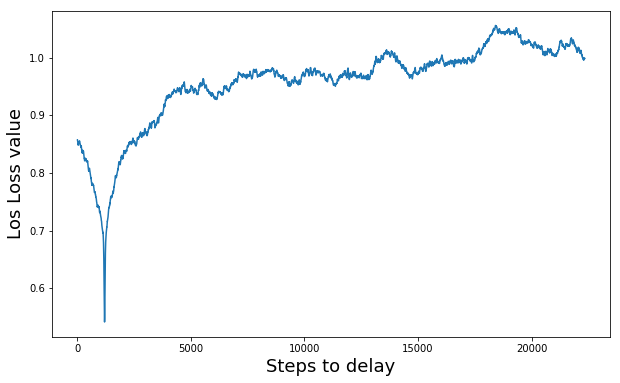
\includegraphics[width=0.4\textwidth]{log_loss_steps_sabater}
	\caption{Log loss plot when matching full audio to full subtitles}
	\label{loss_sabater}
\end{wrapfigure}
Using dynamic programming to take account of the fact that every step must be evaluated across the signal, this process took 45 seconds for a tv show and 2 minutes for a film, the whole process using CPU’s. 
This approach is promising and formed the basis upon which this study was formed. There were key differences in the aim that require further study in order to implement this in a live setting.  Since this was performed on the recorded data rather than a live recording, the signals are pure and contain no significant noise, and so a model that could handle such settings needed to be identified. Furthermore, there would be more uncertainty in the start times of the film which would need to be accounted for – search can commence from the beginning and match the 2 full arrays since the aim is to match the full sound track with the subtitle track (with less concern for excessive processing time), whereas in real time, access to the sound track would occur incrementally as new audio is recorded. The Sabater study was informal, with the results released as a blog post and so lacked rigorous (or at least reporting of the) approach and testing environment, with no account of the relative complexities and possible different approaches that could be taken. \newline

A similar approach was adapted in \cite{Ortega2009} in order to align a draft script with a live presentation which loosely followed this but often presented changes in the script and its chronology (insertions, substitutions and deletions). To do so, 12 order MFCC’s were used again, and “normalised energy coefficient augmented by the corresponding delta and delta-delta coefficients information as features”(p2), but an ASR engine formed of “continuous HMMs with context dependent acoustic units, where each unit is modelled with a 16 component Gaussian Mixture Model with diagonal covariance matrices” was used. The HMM’s enable sequence data to be modelled and are not constrained in the same way as RNN’s that must take multiple sequential samples in order to predict a sample, thereby reducing the accuracy achievable. This was a more ambitious objective in that the audio had not been prerecorded and so to compare the audio to the subtitles, the MFCC’s were compared to a phoneme network in order to identify utterances and therefore alignment of the tracks. In addition, this system substituted automatically generated subtitles when no script was available due to insertions.
This model achieved an accuracy of up to 100\% on newscasts that adhered strictly to the script and naturally dropped to 30\% when the programme became unscripted. In addition, due to the preprocessed nature of the scripts the latency was deemed to be negligible. 
Another approach that has been implemented \cite{Campbell1996} In which audio is generated from text by Text To Speech (TTS) systems and this is used to synchronise the text and audio. This is a very promising idea and in the context of this paper’s problems would eliminate the requirement to have the film audio for training, and only the srt. Therefore the aim will be to extend the study to evaluate this method in the noisy setting.
% Chapter 2

\chapter{Preprocessing} % Main chapter title

\label{Chapter2} % For referencing the chapter elsewhere, use \ref{Chapter1} 

%----------------------------------------------------------------------------------------

% Define some commands to keep the formatting separated from the content 
\newcommand{\keyword}[1]{\textbf{#1}}
\newcommand{\tabhead}[1]{\textbf{#1}}
\newcommand{\code}[1]{\texttt{#1}}
\newcommand{\file}[1]{\texttt{\bfseries#1}}
\newcommand{\option}[1]{\texttt{\itshape#1}}

%----------------------------------------------------------------------------------------

\section{Audio Format}
It was deemed most appropriate to use the compressed MP3 extracted from the MPEG-4 video file for a number of reasons. Although using the uncompressed wav form would present a more faithful reproduction of the audio, and possibly provide more data to train on, the additional complexity far outweighed any possible gains. The MFCC extraction is very sensitive to the [something] and testing on the wav file proved prohibitively long. The space requirements were far larger and approached the file size of the compressed video and audio combined. Furthermore, since the aim is to identify human speech, the lossy mpeg compression regime is explicitly designed to mimic the constraints on human hearing using psychoacoustic modelling, whereby imperceptible frequency ranges, signals with subthreshold amplitudes and frequencies masked by other more dominant frequencies are excluded (Perceptual Coding of Digital Audio), among many other filtering techniques. This process is well-suited to feature extraction for ASR as human speech is naturally adapted to be comprehended by human ears, and vice versa. 

The  spoken  voice  frequency  lies between  300  to  3400  Hertz\cite{Sandanalakshmi} and so telephones sample at 8kHz in order to satisfy the nyquist criterion which defines the sample rate necessary to avoid aliasing, where the sample rate frequency is insufficient to capture the full details of the waveform, to be: $f_{s} > 2B$ (sampling frequency greater than twice the bandwidth). 
The sample rate was chosen to be 16kHz in order to avoid this phenomenon, and since the files are compressed the memory requirements are not excessive.

%----------------------------------------------------------------------------------------

\section{Mel Frequency Cepstral Coefficients}

In order to extract the features most relevant to speech, MFCC’s were chosen due to their robustness to noise compared to another popular feature extraction technique, Linear Predictive Cepstral Coefficient \cite{lpccvsmfcc}. Others have found that it performs less well without some preprocessing but is relatively fast to compute \cite{Shrawankar2013}. MFCC’s are considered the baseline, reliable method and there is a python library (python\_speech\_features) available for computing these, and so this was the method chosen.
This technique also applies pschoacoustic modelling to the signal by applying a series of transformations. 

\begin{figure}[h]
	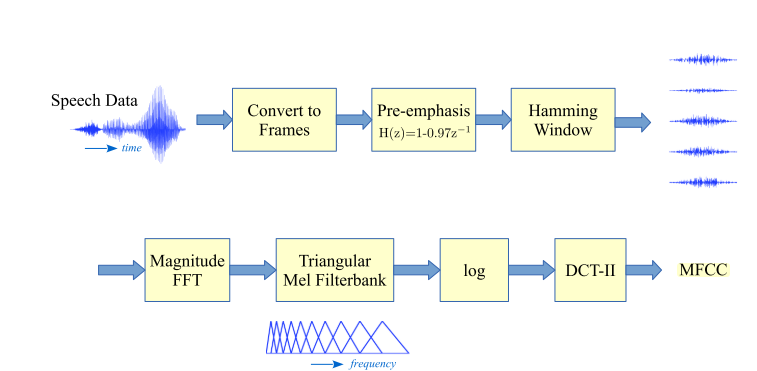
\includegraphics[width=\textwidth]{MFCC_Process}
	\caption{Steps of MFCC Feature Extraction \cite{mfcc_steps}}
	\label{mfcc}
\end{figure}

\subsection{Frame signal into short frames}
The signal is framed into overlapping frames in order for the frequency analysis to be performed. This is assumes that audio spectra are effectively constant over short time frames (typically 20-30ms, ). The windows are overlapping so that continual frequency features are captured...

\subsection{Pre-emphasis}
There is a preemphasis applied, where for each value in the frequency domain a high-pass filter is applied:
\begin{equation}
s_{2}(n) = s(n) - a*s(n-1) 
\end{equation}
where n is the sample number, s is the signal in the frequency domain and s2 is the transformed signal. 
This has 3 effects http://haythamfayek.com/2016/04/21/speech-processing-for-machine-learning.html:
(1) balance the frequency spectrum since high frequencies usually have smaller magnitudes compared to lower frequencies,
(2) avoid numerical problems during the Fourier transform operation and
(3) may also improve the Signal-to-Noise Ratio (SNR).

\subsection{Periodogram}
For each frame the periodogram is calculated, which encapsulates the relative energy in different frequency bands of the signal. This is done using the Discrete Fourier Transform (discrete due to the digital nature of the signal):
\begin{equation}
S_{i}(k) = \sum_{n=1}^{N}  s_{i}(n)h(n)e^{-j2\pi kn/N} \text{for } 1 \leq k \leq K
\end{equation}
where $h(n)$ is an $n$ sample long analysis window (e.g. hamming window), and $K$ is the length of the FFT. For a 16kHz signal in 25ms frames, N equates to 400 samples.
The periodogram-based power spectral estimate for the speech frame  is then given by:
\begin{equation}
P_{i}(k) = \frac{1}{N}|S_{k}|{2}
\end{equation}
i.e. we take the absolute value of the complex fourier transform of each coeffecient, and square the result.

\subsection{Mel Filterbank}
This step applies a series of filters (26 commonly) to the periodogram, composed of vectors of length 26 with nonzero values at different sections along the vector.  The filters are nonuniform, increasing in width with frequency. This emulates the nature of human hearing to have lower sensitivity to changes in frequency as frequency increases. This is based on the Mel scale which models this nonlinearity and describes exactly how to space the bins.
The spectrum $P(f)$ is warped along its frequency axis $f$ (in hertz) into the mel-frequency axis as $P(M)$, where $M$ is the mel-frequency, using:
\begin{equation}
M(f) = 2595 \log((1 + f/700)
\end{equation}
A non-linear frequency scale transformation is applied based on the observation that human hearing does not perceive frequencies linearly but, like amplitude, on a logarithmic scale:
\begin{figure}[h]
	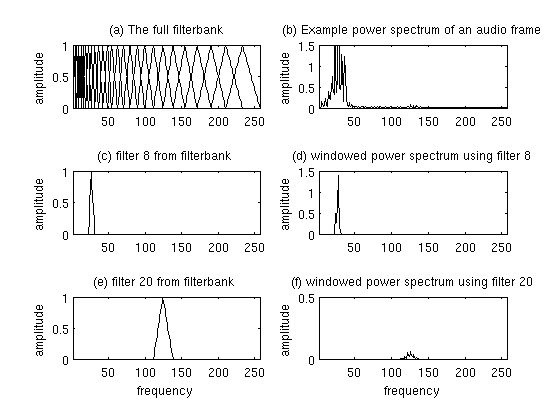
\includegraphics[width=\textwidth]{mel_filterbank_example}
	\caption{Filtering with Mel Filterbanks \cite{practical_cryptography}}
	\label{filterbank}
\end{figure}

\subsection{Log and DCT}
The log of the energies in each filterbank is taken, and a Discrete Cosine Transformation (DCT) is applied to extract 13 new coefficients of this new spectrum. The DCT has several benefits over another transformation like the Fourier transform in that it does not interpret components as infinite waves, and so is better suited where signals are more likely to be interrupted, as the framing process does. Furthermore only real numbers are output which is more readily dealt with by learners such as CNN’s. 
\newline
Generally the largest 13 coefficients are taken that represent the most important information.
https://dsp.stackexchange.com/questions/31/how-do-i-interpret-the-dct-step-in-the-mfcc-extraction-process 
probably need better source…

\subsection{Output}
Hence MFCC’s function as a feature selection technique that reduces the 400 samples each with 256 values ( 8 bits) of amplitude representation to this lower feature space specifically designed to emulate how humans hear, which are themselves well placed to interpret speech signals. However, Figure \ref{mfccs_speech_orno} indicates that the relation between MFCC's and speech presence is not immediately obvious. MFCC2 appears to have the most distinctive correlation with the coefficients doubling in size from $\sim$30 to $\sim$60 in the absence of speech, but other features have similar values, and there is significant intraclass variation.

\begin{figure}[h]
	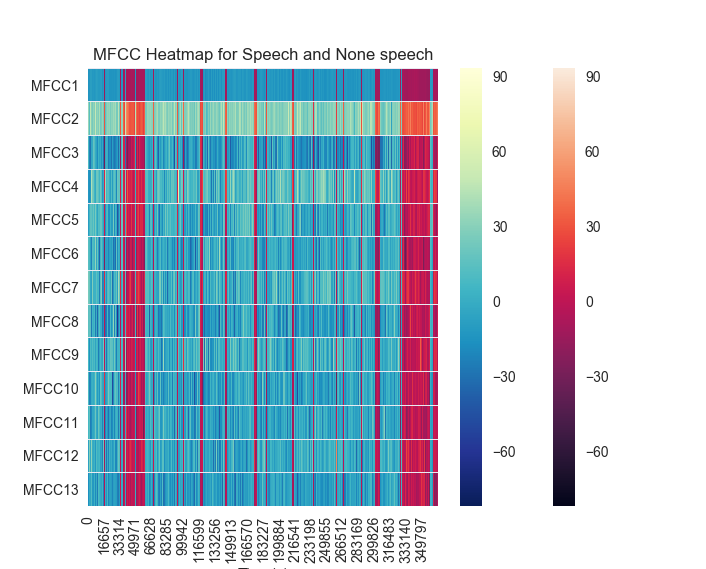
\includegraphics[width=\textwidth]{mfcc_heatmap_speech_or_nospeech}
	\caption{The MFCCs extracted from a Game of Thrones episode. Bluish shades indicate subtitles are absent, pinkish shades indicate they are present. Feature window index is used as a proxy for time.}
	\label{mfccs_speech_orno}
\end{figure}

\section{Subtitles}
The MFCC’s provide the descriptive variables upon which to make predictions, and the objective variable is defined to be the presence of subtitles. This setup was chosen to enable the model to provide based solely on the srt file: since this subtitle synchroniser is aimed principally at cinemagoers, it is assumed that the original audio/video is unavailable, but it is assumed that an srt file is accessible. These are readily available on the internet for most films and are small (essentially text) files and so networking and device requirements would be minimal: they contain a series of entries made up of a start time, stop time, and a string to be presented on the screen at these times. In order to generate the subtitle array:
\begin{itemize}
	\item Times are converted into seconds from start.
	\item The time at which the last subtitle disappears from the screen is used to determine the length in seconds that subtitles are present. Subtitles need only be synchronised when there are actually subtitles present.
	\item The number of frames required is determined by dividing the length in seconds by the frame step (10ms) (the frame length is 25ms, but these are overlapping).
	\item An array of zeros pb\_array is generated with columns for an index, start time and binary subtitle value to indicate presence of subtitles. It is of equal length to the number of frames required.
	\item The 2 arrays, pb\_array and subs\_array, are parsed concurrently, with the frame times of pb\_array checked to see if they lie within a times entry, and the value changed to 1 from 0 if true.
\end{itemize}

\subsection{Pseudocode}
\begin{algorithm}
	\caption{pb\_array\_fill}\label{euclid}
	\begin{algorithmic}[1]
		\Procedure{MyProcedure}{}
		\State $i \gets 0$
		\State $j \gets 0$
		\State $m \gets pb\_array\_length$
		\State $n \gets subs\_array\_length$
		\While {True}
		%\Procedure{Check arrays not exceeded}
		\If {$i > m$ }  
			\BREAK
			\EndIf
		\If {$j > n$ }  
			\BREAK
			\EndIf
		\If {\textit{pb\_array[i] start time} $\geq$ \textit{subs[j] start time}} 
			\If  {\textit{pb\_array[i] end time} $<$ \textit{subs[j] end time}}
				%\COMMENT {Within subs entry}
				\State $pb\_array[i] \gets 1$
				\State $i \gets i+1$
				\EndIf
			%\ELSEIF {$pb\_array[i] end time} $>$ \textit{subs[j] end time}}
			\Else
				\State $j \gets j+1$
			\EndIf
		\EndIf
		\EndProcedure
	\end{algorithmic}
\end{algorithm}

This method was evaluated with 5 trial runs on 59:18 minutes of audio, equating to 355,830 MFCC samples and took on average 12.03 seconds. This is a little longer than would be desired in practice but is not excessively long. This method is efficient in that it parses over the arrays only once.

This outputs a vector with length equal to number of MFCC frames, filled with binary values indicating presence of subtitles. This provides the objective feature to predict.

%----------------------------------------------------------------------------------------

 
% Chapter 3

\chapter{Learning} % Main chapter title

\label{Chapter3} % For referencing the chapter elsewhere, use \ref{Chapter1} 

%----------------------------------------------------------------------------------------

\section{Learner Architecture}
The network architecture implemented by Sabater was used as a starting point. This used convolutions in 1d with kernel size 3, where the filter is initially applied over the MFCC features. This process is identical to the more traditional 2d convolutions in computer vision, except the kernel is a vector rather than a square/array. 3 filters were used.
\begin{wrapfigure}{r}{0.3\textwidth} 
	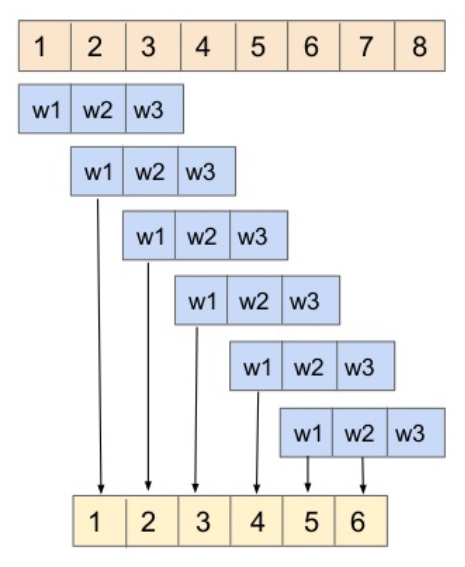
\includegraphics[width=0.3\textwidth]{1dconv_nopad}
	\caption{Convolutions in 1d \cite{catalunya_2017}}
	\label{1dconv}
\end{wrapfigure}
This architecture associates adjacent MFCC’s with each other in a hierarchical fashion. It could be hypothesised that during speech the changes in pitch/frequency occur in a consecutive fashion, with sudden changes from different parts of the spectrum unlikely, and so this information can be compressed/summarised… No padding was used, and although this means central coefficients are over represented in relation to those at the edges, it could also be hypothesised that these occur less often and, being at the edges of the frequency spectrum, are less critical to comprehension, thus features can be reduced further. As in 2d convolutions, the exact nature of the filters are left to be learned during the optimisation (back propogation?) process. 12 filters in 2 convolution layers gives 24 parameters to be learned.
The 1D convolutions output tensors of shape (V-(F-1),NF ), V is the feature vector size, NF is number of filters. To produce the correct shape for the dense layer, the tensors are flattened out to feature vectors again. In the original implementation by Sabater, he applies the ReLu activation function at this point, before applying batch normalisation and dropout. These layers are then repeated until the output neuron with a sigmoid activation function. 
%----------------------------------------------------------------------------------------
\subsection{Activation Functions}
The activation functions provide the mathematical function that emulates the nonlinear, biphasal response in the brain. For all the internal layers the ReLU function was used as this is less computationally expensive than the sigmoid where all neurons are guaranteed to fire at all times, and the use of a dropout layer removes these dying neurons to give a sparser output. 
The output activation function was a sigmoid, which is well suited for classification and ensures that all outputs from the final dense layer will be evaluated.

\begin{figure}[h]
	\centering
	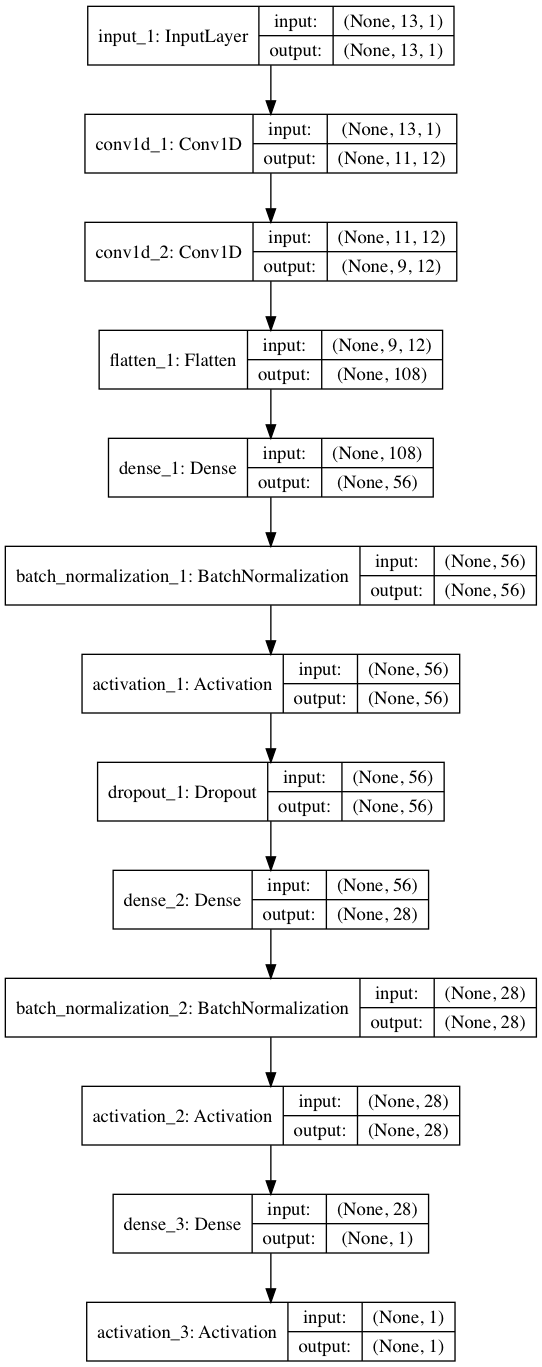
\includegraphics[height=\textheight]{model_plot_normswap}
	\caption{Model Architecture}
	\label{architecture}
\end{figure}

\subsection{Batch Normalisation}
I didn’t normalise the features directly since this relies on having the full dataset and when deployed it would not be possible to do this since we are only granted access to the dataset incrementally.
In order to learn, it is most effective when the training and test data have the same distribution. However, at each layer the outputs retain this relation only weakly due to the non-linearity of the activation functions, a process known as “internal covariance shift”, and so at each layer the new distribution must be relearnt. In addition, due to the flattening of the sigmoid function at larger values, the optimisation process slows as the gradient varies less over fixed learning rates. This can be compensated for by renormalising after every layer, but In order to normalise, the mean and variance is computed across the whole training set, but this is expensive and “not differentiable everywhere”. Instead, batchnorm stochastically computes the mean and variance over much smaller overlapping batches. This can be seen as having a regularising effect as the outputs through each layer are now dependent on what other examples were present in that batch via the mean and variation with which it is normalised rather than being processed independently. Since this process can be done several times, a single example can be related to many other examples. At test time, the learned features of the gaussian are fixed and applied to the data to give deterministic responses.
In order to compensate for this, the outputs can be normalised to a gaussian with zero mean and unit variance across each of the dimensions, output xhat. In order to ensure that the activation functions are thus not constrained to this gaussian distribution, a further transformation is made: $y = \gamma  \hat{x} + \beta$, and incorporate these new parameters into the learning process to be identified via backpropogation, hence different distributions can be inferred directly.

\subsection{Dropout}
Dropout is one method of limiting overtraining and the interdependence of neurons within layers. Nodes are defined to be active in a stochastic function as determined by a probability parameter. Hence when training, every time a sample is propagated through the network a random subset, in proportion to the probability parameter, of the neurons will not produce any output. Hence, later layers cannot depend on the presence of all inputs and reduces the tendency of neurons to co-adapt, activating in similar ways to other neurons and hence not providing additional information. In this way, a much larger set of network configurations is randomly sampled, and hence can be viewed as operating as an ensemble method for 1 hidden layer, different for more than 1.. All architectures share weights – whenever we use a hidden unit its got the same weights as it has in other architectures. Extreme form of bagging – very large number of architectures trained on just 1 sample. Sharing of weights means that every model is very strongly regularised – the weights learned from 1 architecture are stored before the architecture is sampled again. A dropout value of 0.2 was applied.

\section{Tuning}
Once the general neural network architecture was decided, there were still a range of hyperparameters to tune. In order to evaluate the effect of different optimisers, batch size and number of epochs, the hyperas package was used. This enables models with different parameters to be evaluated and the optimal parameters identified using grid search cross validation and an optimisation algorithm, Tree of Parzen Estimators (TPE) was used here. http://hyperopt.github.io/hyperopt/.
The range of parameters tested was: 
batch\_size=[32, 64, 128],
epochs=[1, 2, 3, 4, 5, 6, 7, 8, 9, 10, 50, 100],
optimizer=['SGD', 'RMSprop', 'Adagrad', 'Adadelta', 'Adam', 'Adamax', 'Nadam'],
In so doing, the best performing parameters were identified to be:
optimiser = Nadam, batch size = 32. [However, due to the random initialisation process this produced different results every time...]
\section{Training/Test Set Size}
\begin{wrapfigure}{l}{0.3\textwidth} 
	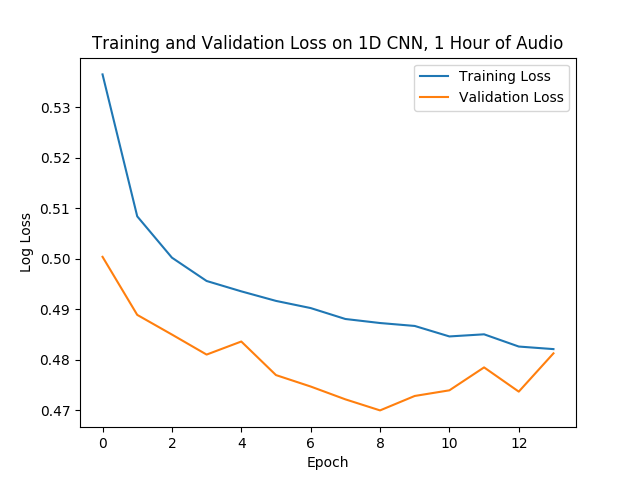
\includegraphics[width=0.3\textwidth]{train_val_loss_run2}
	\caption{Validated on a separate episode of The Walking Dead}
	\label{val_loss}
\end{wrapfigure}
In order to identify the size of training set required, the optimised learner was run on a separate validation set and the loss evaluated with epoch to see how training accuracy would improve with more data. What was thought to be a small dataset consisting of 1 hour of audio from The Walking Dead in fact was enough for the log-loss plot to indicate that the best results achievable had already been done so, and no more data would be required to replicate the results on data with a similar distribution.
Interestingly the validation loss is less than the training loss..
The validation results gave [0.81, 0.50] [accuracy, loss], which emulated closely the training results. This indicated that an hour of audio should be sufficient, but to ensure success, a full feature film was used for training.

\section{Test Time}
Prior to tuning, the model achieved respectable results Validation Loss: 0.47
Validation Accuracy: 0.76
Time:  $\sim103$ seconds

After tuning, these results were improved slightly:
Validation Loss: 0.48
Validation Accuracy: 0.81

The model was then evaluated on a full feature film, Goldstone and produced similar results:

Validation Loss: 0.49
Validation Accuracy: 0.84
Time: $\sim259$ seconds

However, there is some debate over the position of the batch normalisation layer and whether it should be placed before or after the activation [sources here], and so the tests were rerun with this swap implemented. 
In doing so, the training time and accuracy were improved significantly

Validation Loss: 0.50
Validation Accuracy: 0.93
Time: $\sim216$ seconds

suggesting better generalisation at test time.

% Chapter Template

\chapter{Synchronising} % Main chapter title

\label{ChapterX} % Change X to a consecutive number; for referencing this chapter elsewhere, use \ref{ChapterX}

%----------------------------------------------------------------------------------------
%	SECTION 1
%----------------------------------------------------------------------------------------

\section{Array Matching}
With a sufficiently accurate subtitle predictor, the next challenge was to match the predictions to the  true array. Sabater initially took the whole prediction array and computed the log loss over different positions of the subtitles array in order to find the minimum which would equate to the best match. However, this approach assumes full access to both arrays: in order to match subtitles in real time, the probability array would be accessed incrementally as new audio is recorded and features extracted. 

\subsection{Fixed Recording Duration}
Initially, it was attempted to record audio of fixed duration in order to match (size 50 initially, equivalent to 500ms), whilst noting the time for the algorithm to run, and applying a delay to the subtitles once the match had been found. The length of the audio was to be optimised, and it was assumed that live audio data would commence acquisition after the beginning of the film so that the algorithm does not attempt to match audio features generated before the film has actually begun, perhaps due to background noise or advertisments. To test this independently of the subtitles predictor, the array match was given a sample of the subtitles array N steps after the beginning of the full subtitles array in order to evaluate the behaviour. Interestingly, this approach consistently returned index 0 as the best position. On investigation, it was revealed that there were no subtitles at the beginning and so the sample array was made up of entirely zeros, and so the function returned this as the optimal spot: there were in fact multiple optimum positions (generally all at the start) where no subtitles were present and it simply returned the first position which fulfilled the minimisation condition. 

\subsection{Live Recording}
Whilst this seemed like an obstacle initially, it was realised that the duration of time in which no subtitles occurs can be considered a distinctive feature in itself, especially when combined with the assumption that synchronisation has commenced not long after the beginning of the film: it is unlikely that viewing would commence after the majority of the film has already finished. In addition, new data can be continuously acquired by simply appending new predictions based on new features extracted from the incoming audio. This foreknowledge, a product of the specific nature of this problem, can be utilised to shrink the search space significantly by defining the first match to be obtimal, whilst continuously expanding the number of examples to match against the base truth. In practice this is implemented by recording data and extracting the features, and if no speech is found, continue to acquire new data until a subtitle is predicted. This subtitle would correspond to the first subtitle present in the film and would provide the distinctive feature to search for when matching. This could be done in 2 ways, either the array generated, of a long sequence of zeros followed by a 1, is matched using the log loss, or in an even greater simplification, the subtitles are simply commenced as soon as this is detected. Alternatively, if speech commences from the beginning, the recorded features should provide enough variation that a match can be found when searching from the beginning.
– the longer the duration of time in which no subtitles occurs, the longer the sequence of zeros 
 
% Chapter Template

\chapter{Conclusions} % Main chapter title

\label{ChapterX} % Change X to a consecutive number; for referencing this chapter elsewhere, use \ref{ChapterX}

%----------------------------------------------------------------------------------------
%	SECTION 1
%----------------------------------------------------------------------------------------
\subsection{Preprocessing}
An efficient means of extracting features from subtitle files has been combined with traditional speech centred feature extraction in order to generate data for training easily.

\subsection{Learner}
A learner has been trained that can identify speech with approximately 80\% accuracy in a range of conditions. This is less than commercial speech detectors which approach 100\% accuracy, but the conditions generally involve much less noise where the speaker is emphasised. The results could possible be improved by appending the log energy to the feature vector, using padding when taking convolutions to ensure all features have equal representation, using noise reduction techniques. Alternative learning frameworks could be evaluated to ensure the highest accuracy possible is attained.

\subsection{Array Matching}
Given a sufficiently accurate model, a means of matching predictions to a true array in real time has been proposed. This attempts to utilise additional information peculiar to the setting of the cinema to restrict the search space. This is effective assuming insignificant speech noise from the surroundings, but requires additional testing in order to identify the most effective sample length to match with when speech is present in the film.



 

%----------------------------------------------------------------------------------------
%	THESIS CONTENT - APPENDICES
%----------------------------------------------------------------------------------------

%\appendix % Cue to tell LaTeX that the following "chapters" are Appendices

% Include the appendices of the thesis as separate files from the Appendices folder
% Uncomment the lines as you write the Appendices

%% Appendix A

\chapter{Frequently Asked Questions} % Main appendix title

\label{AppendixA} % For referencing this appendix elsewhere, use \ref{AppendixA}

\section{How do I change the colors of links?}

The color of links can be changed to your liking using:

{\small\verb!\hypersetup{urlcolor=red}!}, or

{\small\verb!\hypersetup{citecolor=green}!}, or

{\small\verb!\hypersetup{allcolor=blue}!}.

\noindent If you want to completely hide the links, you can use:

{\small\verb!\hypersetup{allcolors=.}!}, or even better: 

{\small\verb!\hypersetup{hidelinks}!}.

\noindent If you want to have obvious links in the PDF but not the printed text, use:

{\small\verb!\hypersetup{colorlinks=false}!}.

%\include{Appendices/AppendixB}
%\include{Appendices/AppendixC}

%----------------------------------------------------------------------------------------
%	BIBLIOGRAPHY
%----------------------------------------------------------------------------------------

\printbibliography[heading=bibintoc]

%----------------------------------------------------------------------------------------

\end{document}  
